% Slide 13: Regression Trees
\begin{frame}{درخت‌های رگرسیون}{\lr{Regression Trees}}
  \begin{itemize}
    \setlength{\itemsep}{2pt}
    \item ایده اصلی یادگیری و به‌کارگیری درخت‌های تصمیم، برای مسائل رگرسیون نیز قابل تعمیم است.
    \item \textbf{تفاوت‌ها با درخت تصمیم در طبقه‌بندی:}
    \begin{enumerate}
      \setlength{\itemsep}{1pt}
      \item \textbf{معیار تفکیک:} تفکیک‌ها با هدف بیشینه‌سازی کاهش خطا (\lr{MSE}) انجام می‌شوند (نه شاخص \lr{GINI}).
      \item \textbf{پیش‌بینی در برگ‌ها:} خروجی هر برگ، میانگین مقادیر نمونه‌های آموزشی حاضر در آن برگ است.
    \end{enumerate}
  \end{itemize}
  \vspace{0.05cm}
  \begin{columns}[c]
    \begin{column}{0.48\textwidth}
      \centering
      {\small\bfseries\color{mannheimblue}درخت رگرسیون \lr{(Regression Tree)}}
    \end{column}
    \begin{column}{0.48\textwidth}
      \centering
      {\small\bfseries\color{mannheimblue}درخت تصمیم \lr{(Decision Tree)}}
    \end{column}
  \end{columns}
  \vspace{0.02cm}
  \begin{center}
    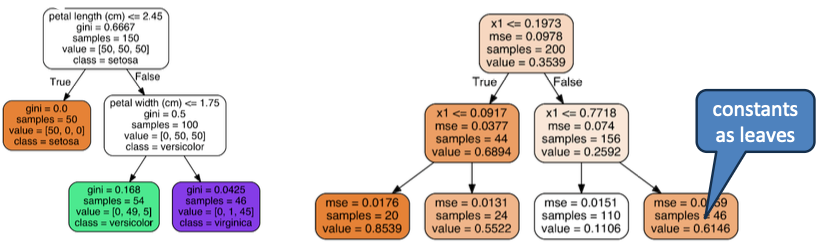
\includegraphics[width=0.96\textwidth,height=2.75cm,keepaspectratio]{images/slide13_trees_comparison_clean.png}
  \end{center}
\end{frame}

% Slide 14: Regression Trees Depth & Partitioning
\begin{frame}{عمق درخت رگرسیون و افراز فضا}{\lr{Regression Trees: Depth \& Partitioning}}
  \begin{columns}[c]
    \begin{column}{0.58\textwidth}
      \begin{itemize}
        \setlength{\itemsep}{4pt}
        \item پارامترهای پیش‌هرس (\lr{Pre-pruning}) میزان برازش درخت با داده‌های آموزشی را مشخص می‌کنند:
        \begin{itemize}
          \item به عنوان مثال پارامتر \lr{\texttt{max\_depth}}.
        \end{itemize}
        \item \textbf{مدل حاصل:} یک \textbf{تابع تکه‌ای-ثابت} بر روی فضای ویژگی‌ها است:
        \begin{center}
          {\small\color{subgray}\lr{Piecewise Constant Function}}
        \end{center}
      \end{itemize}
    \end{column}
    \begin{column}{0.40\textwidth}
      \begin{center}
        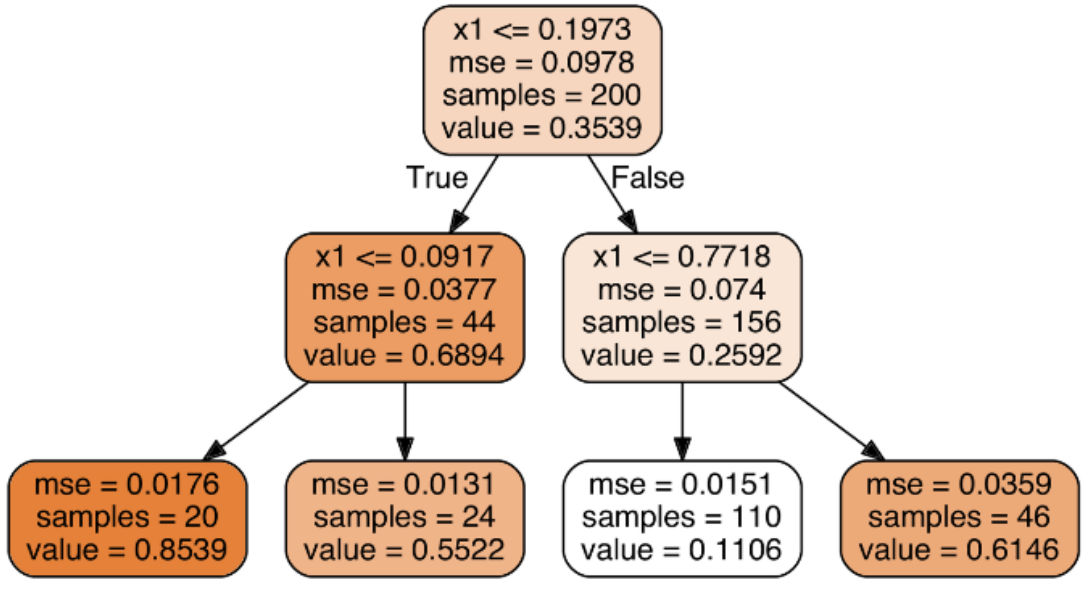
\includegraphics[height=2.0cm,keepaspectratio]{images/slide14_depth_tree.png}
      \end{center}
    \end{column}
  \end{columns}
  \vspace{0.1cm}
  \begin{center}
    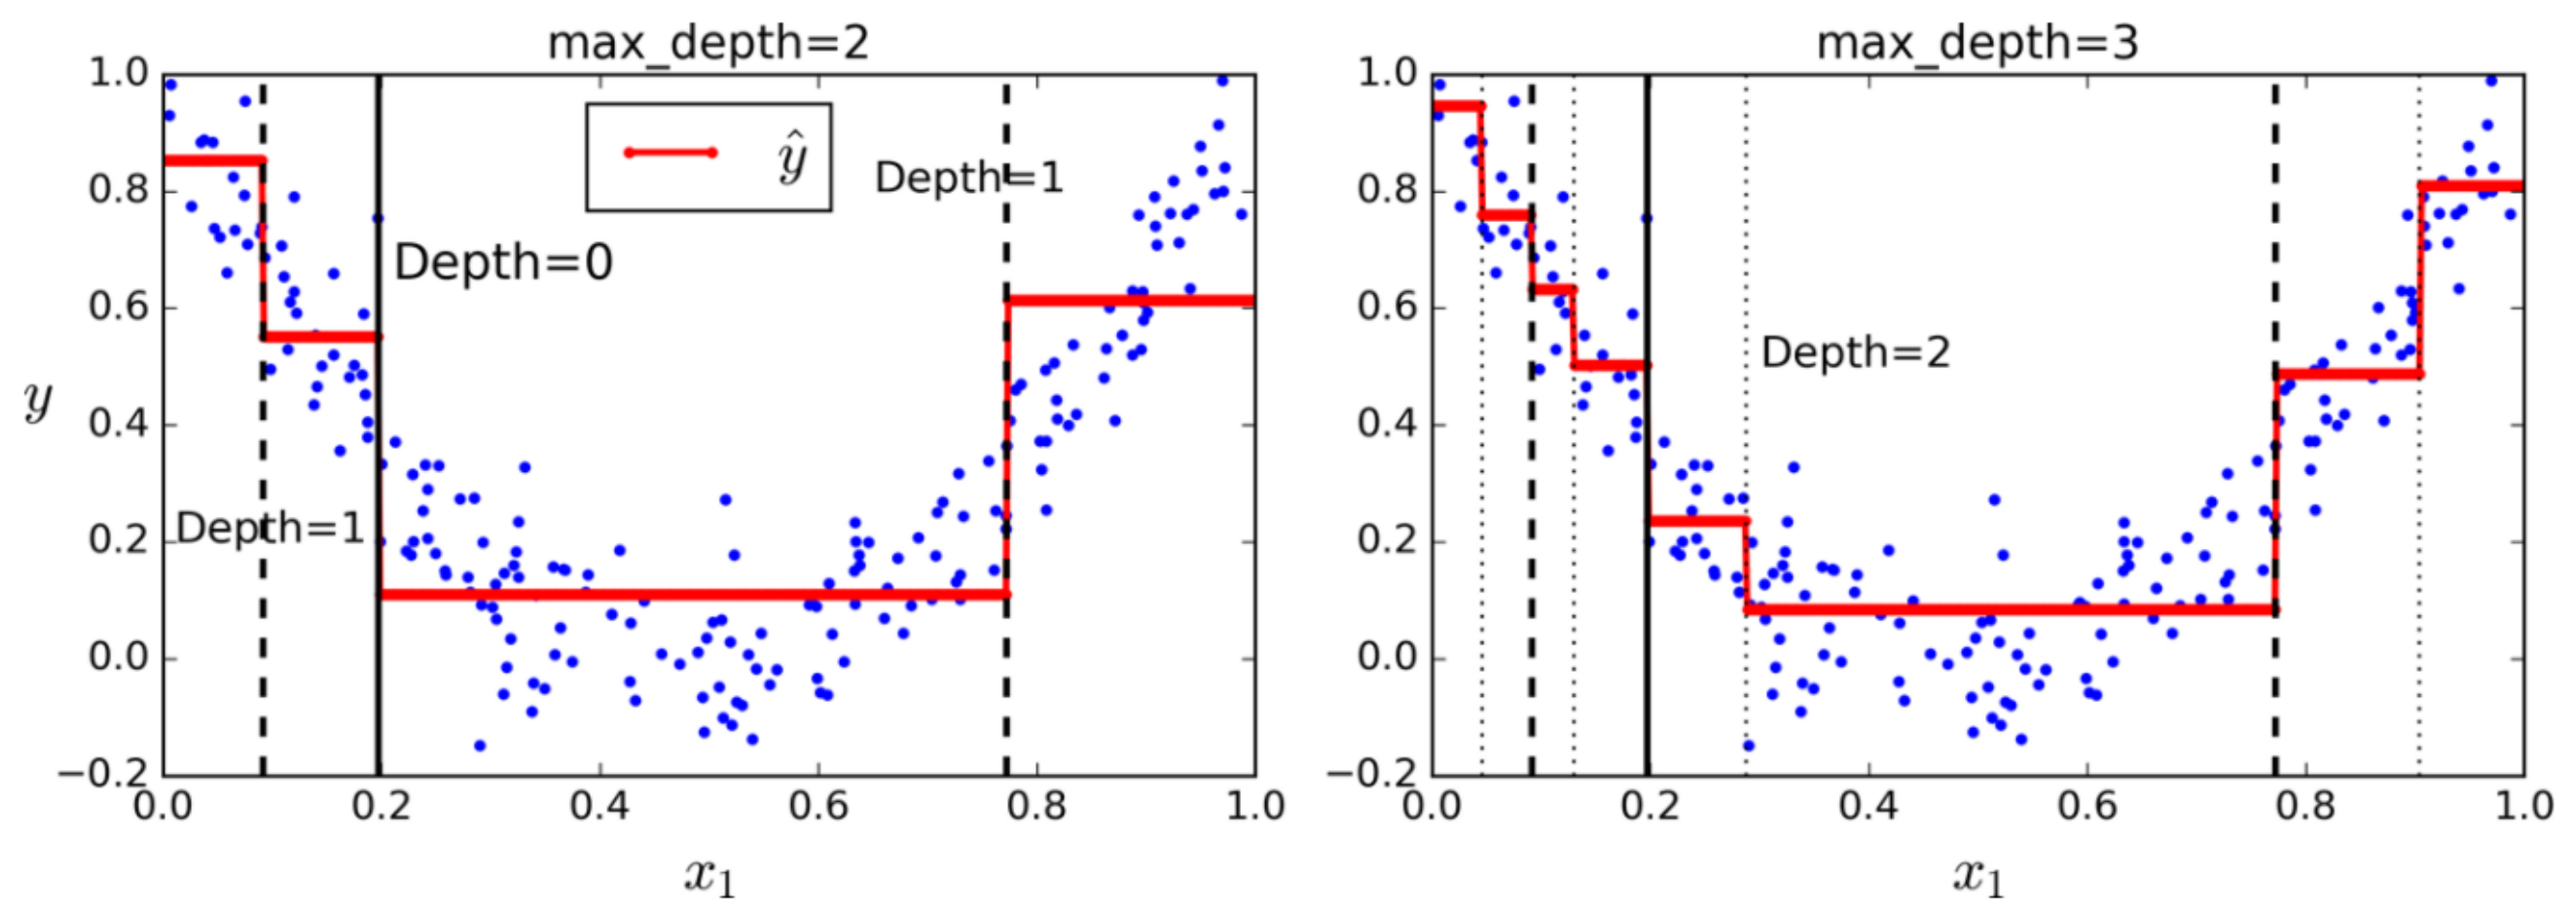
\includegraphics[width=0.95\textwidth,height=2.3cm,keepaspectratio]{images/slide14_tree_partition.png}
  \end{center}
\end{frame}

% Slide 15: Model Trees
\begin{frame}{درخت‌های مدل}{\lr{Model Trees}}
  \begin{columns}[T]
    \begin{column}{0.52\textwidth}
      \begin{itemize}
        \setlength{\itemsep}{5pt}
        \item \textbf{ایده:} تفکیک اولیه داده‌ها به شکلی که ارتباط در هر بخش «خطی‌تر» شود.
        \begin{itemize}
          \item \textbf{مثال:} مصرف سوخت بر حسب وزن خودرو.
        \end{itemize}
        \item \textbf{به جای مقدار ثابت در هر برگ:} یک تابع رگرسیون خطی آموزش داده می‌شود.
        \item \textbf{نحوه پیش‌بینی:} پیمایش ساختار درخت تا رسیدن به برگ متناظر، سپس ارزیابی تابع رگرسیون همان برگ.
        \item \textbf{مدل حاصل:} \textbf{تابع تکه‌ای-خطی (\lr{Piecewise Linear})}.
      \end{itemize}
    \end{column}
    \begin{column}{0.46\textwidth}
      \begin{center}
        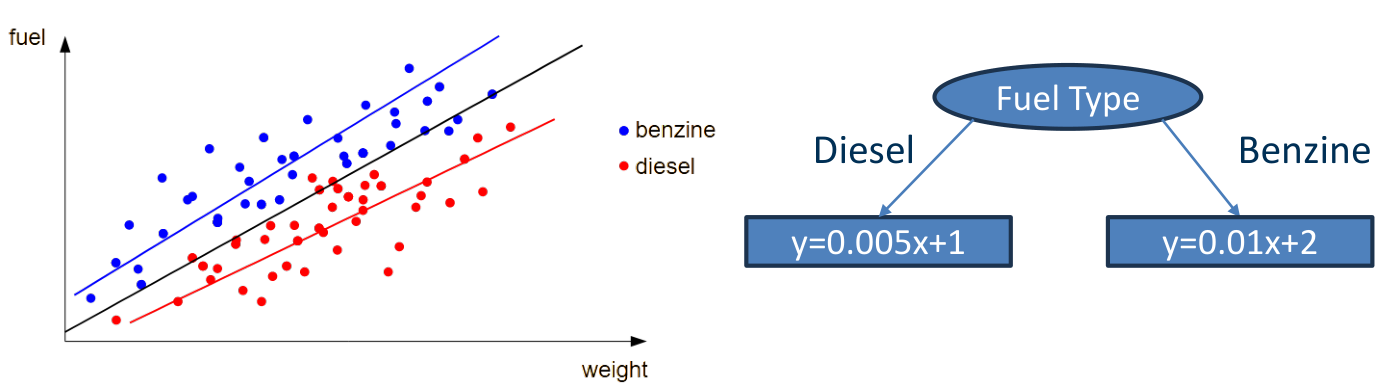
\includegraphics[width=\textwidth,height=4.2cm,keepaspectratio]{images/slide15_model_tree_plot.png}
      \end{center}
    \end{column}
  \end{columns}
\end{frame}
